\chapter{Conception}
\label{chap:Conception}
  Ce chapitre présente l'architecture pensée pour la mise en \oe{}uvre d'un
  éditeur collaboratif utilisant \emph{Logoot} comme CRDT\footnote{Commutative
  Replicated Data Types}. La figure \ref{fig:architecture} représente cette
  architecture et sert de support aux explications qui suivent.

  \begin{figure}[hbt]
    \label{fig:architecture}
    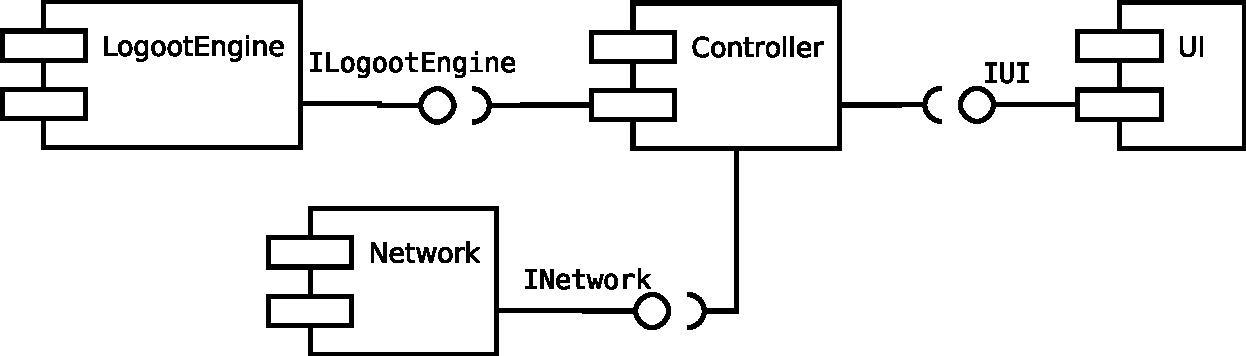
\includegraphics[width=\textwidth]{includes/architecture.pdf}
    \caption{Architecture d'un éditeur collaboratif utilisant \emph{Logoot}}
  \end{figure}

  Dans la suite de ce chapitre nous détaillons chaque composant et les
  interfaces qui les accompagnent.

  \section{LogootEngine}
  \begin{figure}[hbt]
    \center
    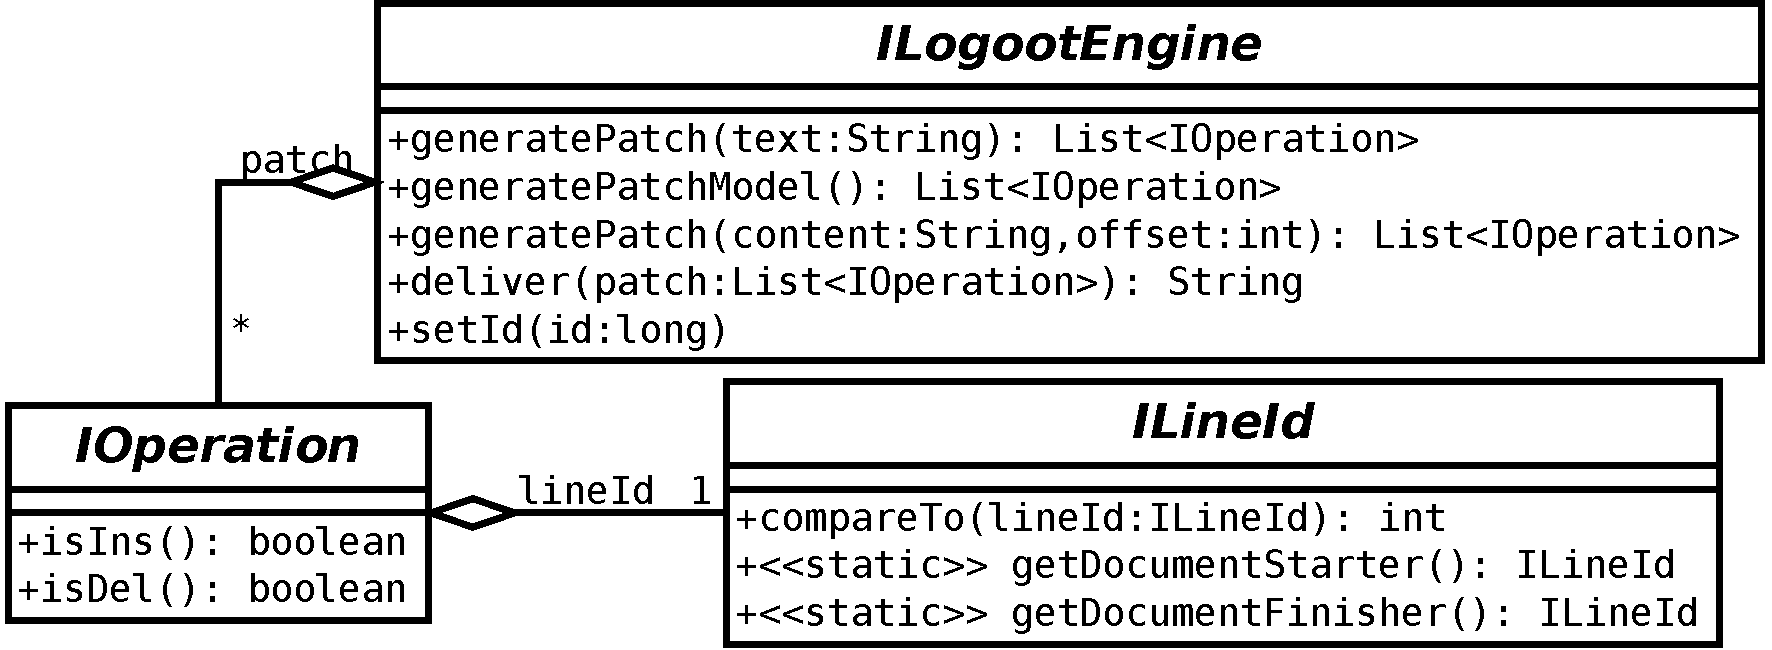
\includegraphics[width=.9\textwidth]{includes/model/ILogootEngine.pdf}
    \caption{Composant \emph{LogootEngine}}
    \label{fig:logootengine}
  \end{figure}

  Le \emph{LogootEngine} (figure~\ref{fig:logootengine}
  page~\pageref{fig:logootengine}) maintient le modèle de texte relatif
  à \emph{Logoot}, c'est-à-dire la table des identifiants. Pour se faire, le
  \emph{LogootEngine} offre les services de génération et d'intégration de
  patch. Un patch étant une liste d'opérations d'insertion et de suppression
  d'identifiants. Le composant \emph{LogootEngine} fourni plusieurs opération
  de générations et d'intégration d'un patch : 
  \begin{enumerate}
    \item L'opération \verb?generatepatchFromModel()? permet de générer un patch
    représentant le modèle. Cette opération est utile lorsqu'un nouvelle
    utilisateur joins l'édition d'un document et qu'il doit charger le
    contexte (les identifiants) du document;
    \item L'opération \verb?generatePatch(text)? génère un patch
    depuis un état précédent du texte grâce à l'algorithme du diff. Bien que
    facile à implémenter, cette opération ralentie fortement l'exécution. Ceci
    est du à l'algorithme du diff qui à une complexité en
    $O(m \times n)$ (avec $m$ le nombre de caractères dans le document sources
    et $n$ le nombre de caractères dans la variable $text$) ;
    \item L'opération \verb?generatePatch(content, offset)? génère un
    patch en fonction d'une insertion ou d'une suppression dans le document
    texte. La génération du patch est nettement plus performante avec une
    complexité temporelle qui est égale à la génération et le maintient de la
    table des identifiants ;
    \item L'opération \verb?deliver(patch)? s'occupe de l'intégration du patch.
    Deux comportements sont possibles. Soit cette méthode retourne le texte
    du document après application des modifications. Soit cette
    méthode retourne uniquement les caractères à insérer / supprimer avec
    leur offset.
  \end{enumerate}

  \section{Network}
  \begin{figure}[hbt]
    \center
    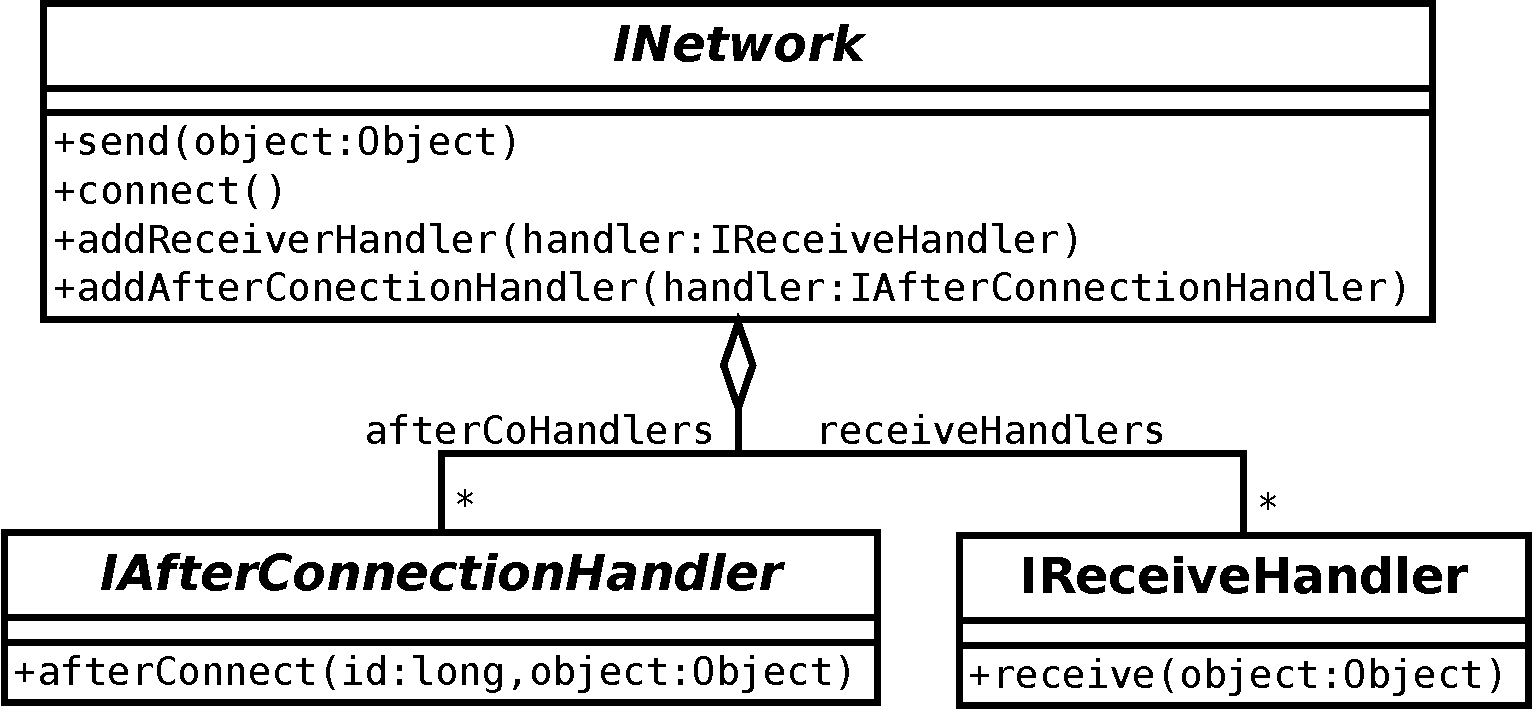
\includegraphics[width=.7\textwidth]{includes/model/INetwork.pdf}
    \caption{Composant \emph{Network}}
    \label{fig:network}
  \end{figure}

  Le composant \emph{Network} (figure~\ref{fig:network}
  page~\pageref{fig:network}) fournit des services d'envoi et de réception de
  données. Il est utilisé pour émettre un patch lors de modifications locales
  du document et pour recevoir les patchs générés par d'autres utilisateurs.
  Pour utiliser les services, l'utilisateur doit au préalable se connecter.
  Le composant \emph{Network} offre plusieurs ouverture où l'utilisateur peut
  définir des fonctions de rappelles. Les \verb?IAfterConnectionHandler? sont
  appelés à la fin de chaque connexion. Les \verb?IReceiveListener? sont appelés
  à chaque réception de données.

  \section{UI}
  \begin{figure}[hbt]
    \center
    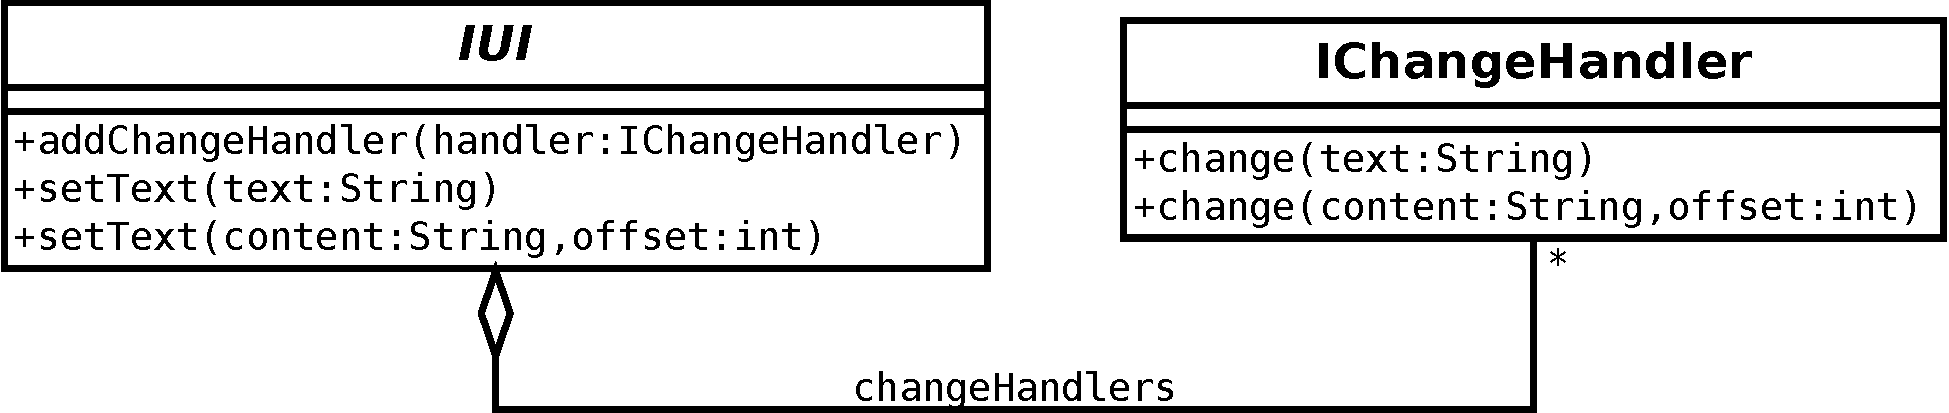
\includegraphics[width=.9\textwidth]{includes/model/IUI.pdf}
    \caption{Composant \emph{UI}}
    \label{fig:ui}
  \end{figure}

  Le composant \emph{UI} (User Interface) (figure~\ref{fig:ui}
  page~\pageref{fig:ui}) représente l'interface
  graphique de l'éditeur. Elle permet à l'utilisateur de visionner et modifier
  un document texte. Pour se faire la méthode \verb?setText(text)? remplace le 
  texte du document et la méthode \verb?setText(content, offset)?
  modifier le document à une position donnée. Le composant \emph{UI} permet
  d'exécuter des fonctions de rappelles après chaque modification du texte (en
  ajoutant des \verb?IChangeHandler? avec l'opération \verb?addChangeHandler?).

  \section{Controller}
  \begin{figure}[hbt]
    \center
    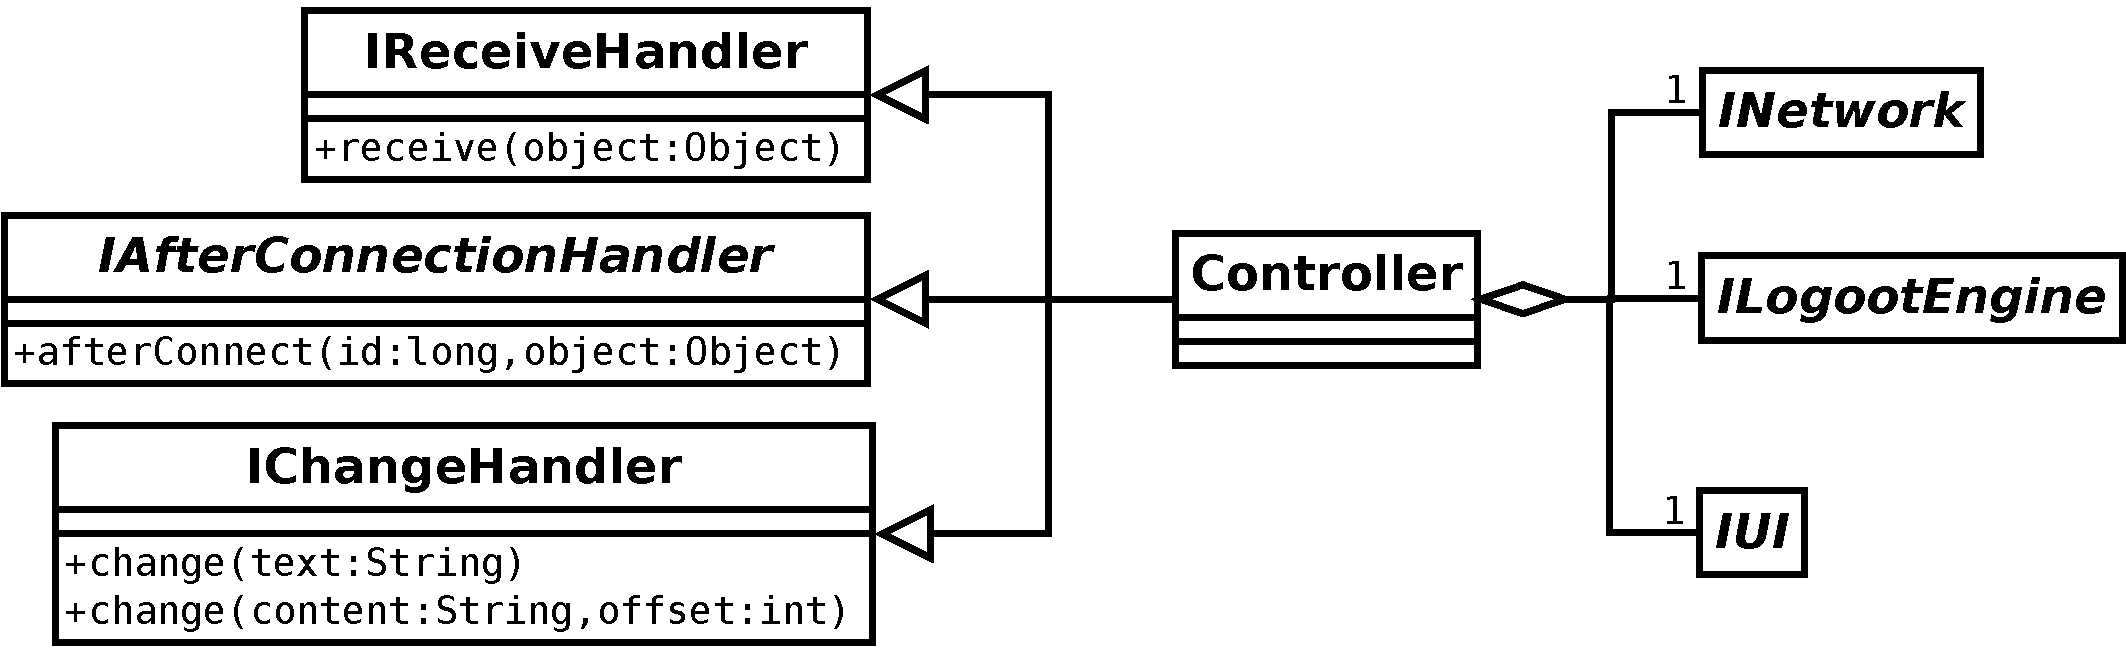
\includegraphics[width=.9\textwidth]{includes/model/Controller.pdf}
    \caption{Composant \emph{Controller}}
    \label{fig:controller}
  \end{figure}

  Le composant \emph{Controller} (figure~\ref{fig:controller}
  page~\pageref{fig:controller}) configure le système. Il demande
  au \emph{LogootEngine} de mettre à jour sont modèle, notifie l'\emph{UI} des
  modifications des autres utilisateurs et envoie les patchs sur le réseau
  grâce au \emph{Network}. Le composant \emph{Controller}
  implémente toutes les interfaces d'handler ce qui lui permet :
  \begin{itemize}
    \item de capter la modification du document texte sur l'\emph{UI} et
    demander au \emph{LogootEngine} de générer un nouveau patch ;
    \item de capter la réception de patchs depuis le \emph{Network} pour les
    faire intégrer par le\emph{LogootEngine} et mettre à jours l'\emph{UI}.
    \item de capter la connexion d'un client sur le \emph{Network} pour récupérer
    un identifiant unique et un patch afin d'initialiser le \emph{LogootEngine} ;
  \end{itemize}

